% Provenance (never printed): cycle 2 "Questionner l'espace et le temps ---
% se situer dans l'espace": representations of familiar spaces (plans), "lire
% des plans, se reperer sur des cartes. Elements constitutifs d'une carte :
% titre, echelle, orientation, legende"; see sources/book1/PROVENANCE.md.
% Book 1, grade 2, chapter 2. Sync 1: "scale" is owned here; "cardinal
% directions" is the physics series' term (prose only); "compass rose" here.
\chapter{从图画到地图}\label{ch:g2:drawing-to-map}

一只鸽子飞过学校上空。它看到了什么？看不到前门，看不到窗户，
也看不到孩子们的脸：从高处往下看，它只能看到东西的顶部。
楼房的屋顶是一块块灰色的长方形。操场是一个大大的空白形状，
上面有几棵圆圆的树冠。小路是细细的线条。
鸽子是从上往下看学校的，就像\omterm{def:g2:drawing-to-map:map}{地图}所画的那样。

\begin{omfigure}
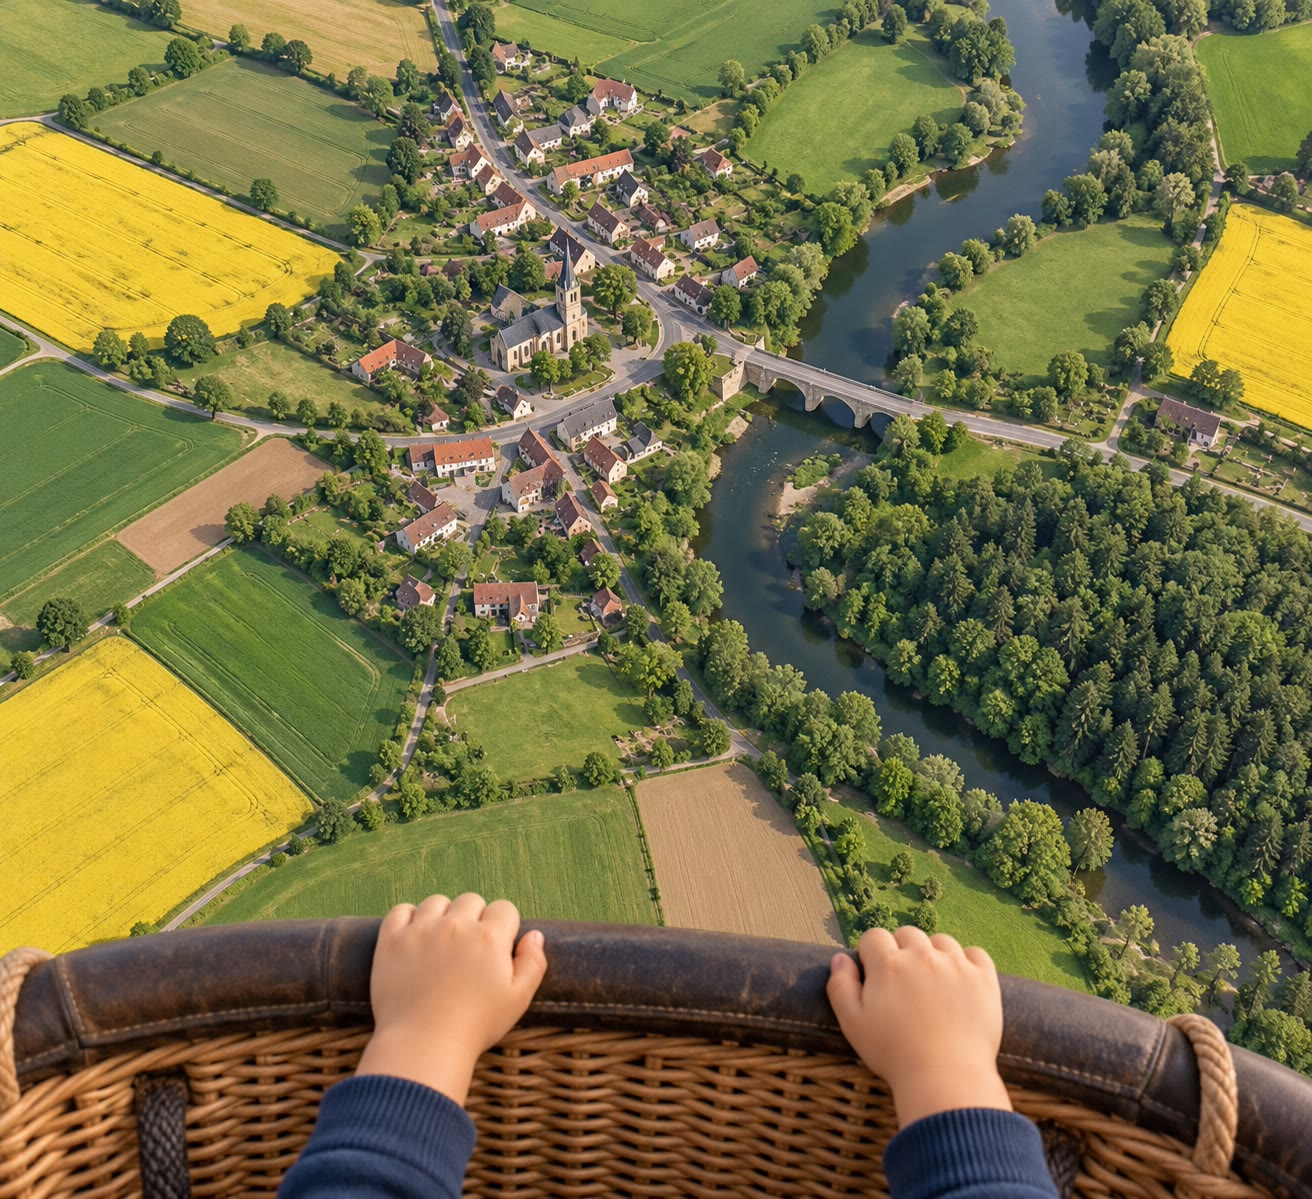
\includegraphics[width=0.62\linewidth]{images/book1/ai/g2-balloon-view.jpg}

{\small 热气球上看到的乡村：田野、村庄、
道路、\omterm{def:g1:landscapes-around-us:water}{河流}及其桥梁，都是从上往下看到的。}
\end{omfigure}

\section{从侧面看与从上面看}

在桌子上放几块玩具积木。从侧面看它们，能看到它们的
高矮，后面的积木被前面的挡住了。
现在站起来，从上往下看它们：看不出它们有多高，
但能看清每一块的确切位置，以及它们之间相隔多远。

\begin{omfigure}
\begin{tikzpicture}[x=1cm, y=1cm, font=\small]
  % side view
  \begin{scope}
    \draw[black!50] (-0.2,0) -- (4.6,0);
    \fill[red!55, draw=black!60] (0.2,0) rectangle (1.2,1.6);
    \fill[ocBlue!55, draw=black!60] (1.6,0) rectangle (3.0,0.8);
    \fill[yellow!70, draw=black!60] (3.4,0) -- (3.9,1.1) -- (4.4,0) -- cycle;
    \node at (2.2,-0.5) {从侧面看};
  \end{scope}
  % from above
  \begin{scope}[shift={(6.4,0)}]
    \draw[black!30, fill=black!3] (-0.2,-0.1) rectangle (4.6,2.3);
    \fill[red!55, draw=black!60] (0.2,0.4) rectangle (1.2,1.4);
    \fill[ocBlue!55, draw=black!60] (1.6,1.0) rectangle (3.0,2.0);
    \fill[yellow!70, draw=black!60] (3.9,0.75) circle (0.5);
    \node at (2.2,-0.5) {从上面看};
  \end{scope}
\end{tikzpicture}

{\small 桌上有三块积木：一块高的红色积木、一块扁平的蓝色积木和一个
黄色圆锥。从上面看，圆锥是一个圆，高的积木是一个
正方形。}
\label{fig:g2:drawing-to-map:blocks}
\end{omfigure}

\begin{definition}[平面图]\label{def:g2:drawing-to-map:plan}
称\emph{平面图}\index{平面图}为从正上方看到的小地方的图，
如一个房间、一座房子、一所学校或一个花园，
它比实际的地方画得小，但每个部分都在正确的位置上。
\end{definition}

\section{画小一点：比例尺}

教室实际太大，不能原样画在一张纸上。我们把它画小，
但每个部分都必须按同样的比例缩小，否则\omterm{def:g2:drawing-to-map:plan}{平面图}就会失真。
最简单的办法是使用方格纸：
方格纸上的一格代表教室里的一米。

\begin{definition}[比例尺]\label{def:g2:drawing-to-map:scale}
\omterm{def:g2:drawing-to-map:plan}{平面图}或\omterm{def:g2:drawing-to-map:map}{地图}的\emph{比例尺}\index{比例尺}，表示图上的长度比实际地方缩小了多少，
也就是图上一段长度在地面上代表多长的实际距离。
例如：\emph{图上 1 格代表实际 1 米}。
\end{definition}

\begin{omfigure}
\begin{tikzpicture}[x=0.75cm, y=0.75cm, font=\scriptsize]
  \draw[black!15] (0,0) grid (10,8);
  \draw[black, line width=1.6pt] (0,0) rectangle (10,8);
  % board on the north wall
  \fill[black!70] (3,7.8) rectangle (7,8);
  % teacher's desk
  \fill[brown!50, draw=black!70] (4,6) rectangle (6,7);
  % pupils' desks: 3 rows of 3
  \foreach \x in {1,4,7} \foreach \y in {1,2.5,4}
    \fill[orange!45, draw=black!70] (\x,\y) rectangle ++(2,1);
  % cupboard
  \fill[ocBlue!40, draw=black!70] (9,5) rectangle (10,8);
  % door (gap) on the east wall, windows on the west wall
  \fill[white] (9.85,1) rectangle (10.15,2);
  \draw[black!70] (10,2) arc[start angle=90, end angle=180, radius=1];
  \foreach \y in {1.5,4.5}
    \draw[ocBlue, line width=2.5pt] (0,\y) -- (0,\y+2);
  % legend
  \begin{scope}[shift={(11,7.2)}]
    \node[anchor=west, font=\small\bfseries] at (0,0.4) {教室};
    \fill[black!70] (0,-0.25) rectangle (0.8,-0.05); \node[anchor=west] at (1,-0.15) {黑板};
    \fill[brown!50, draw=black!70] (0,-1.1) rectangle (0.8,-0.7); \node[anchor=west] at (1,-0.9) {教师桌};
    \fill[orange!45, draw=black!70] (0,-1.85) rectangle (0.8,-1.45); \node[anchor=west] at (1,-1.65) {学生桌};
    \fill[ocBlue!40, draw=black!70] (0,-2.6) rectangle (0.8,-2.2); \node[anchor=west] at (1,-2.4) {柜子};
    \draw[ocBlue, line width=2.5pt] (0,-3.15) -- (0.8,-3.15); \node[anchor=west] at (1,-3.15) {窗户};
    \draw[black!70] (0.8,-3.95) arc[start angle=0, end angle=90, radius=0.6]; \draw[black, line width=1.6pt] (0.2,-3.95) -- (0.8,-3.95); \node[anchor=west] at (1,-3.7) {门};
    \draw[black!15] (0,-4.9) rectangle (0.75,-4.15);
    \node[anchor=west] at (1,-4.53) {1 格 = 1 米};
    \pic[scale=0.7, transform shape] at (0.7,-6.2) {compassrose};
  \end{scope}
\end{tikzpicture}

{\small 方格纸上的教室\omterm{def:g2:drawing-to-map:plan}{平面图}，附有图名、
\omterm{def:g2:drawing-to-map:legend}{图例}、\omterm{def:g2:drawing-to-map:scale}{比例尺}和\omterm{def:g2:drawing-to-map:directions}{罗盘玫瑰}。北墙（有黑板的一面）
位于图的上方。}
\label{fig:g2:drawing-to-map:classroom}
\end{omfigure}
% (exercise data: an invented classroom of 10 m by 8 m)

\begin{method}[在平面图上测量]\label{met:g2:drawing-to-map:measure}
要在方格纸画的\omterm{def:g2:drawing-to-map:plan}{平面图}上求实际长度：
\begin{enumerate}
  \item 数出要测量的那段长度上有几个方格；
  \item 读\omterm{def:g2:drawing-to-map:scale}{比例尺}：每个方格代表多少；
  \item 答案用米表示（\omterm{def:g2:drawing-to-map:map}{地图}上也可用千米）。
\end{enumerate}
\end{method}

\begin{example}[教室有多长？]\label{ex:g2:drawing-to-map:length}
\omterm{def:g2:drawing-to-map:plan}{平面图}的北墙上有 10 个方格。每个方格代表
1 米，所以教室长 10 米。西墙上有
8 个方格，即宽 8 米。黑板占北墙的 4 个方格，
即长 4 米。
\end{example}

\begin{omfigure}
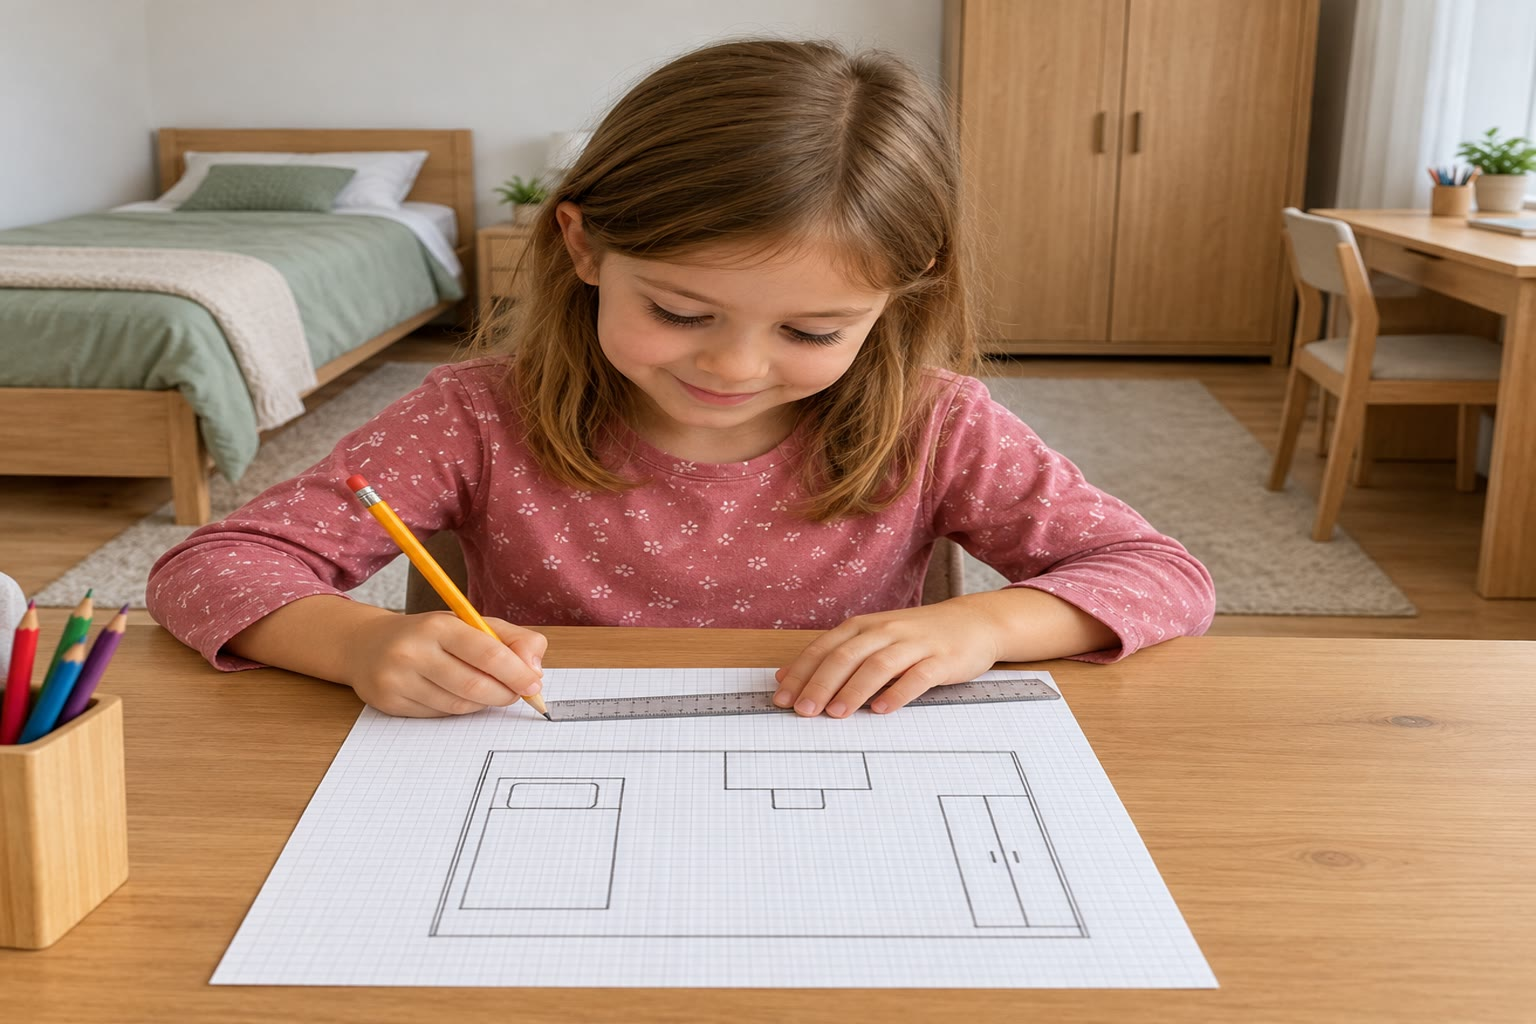
\includegraphics[width=0.55\linewidth]{images/book1/ai/g2-bedroom-plan.jpg}

{\small 在方格纸上画出卧室的\omterm{def:g2:drawing-to-map:plan}{平面图}。}
\end{omfigure}

\section{从平面图到地图}

\omterm{def:g2:drawing-to-map:plan}{平面图}画的是一个小地方。当我们要画一个更大的地方——例如整个城镇、
一个\omterm{def:g1:landscapes-around-us:landform}{山谷}、一个国家——就要画\omterm{def:g2:drawing-to-map:map}{地图}。

\begin{definition}[地图]\label{def:g2:drawing-to-map:map}
称\emph{地图}\index{地图}为地球表面大片区域的图画，
它从上往下看，并且画得比实际小得多。
\end{definition}

在\omterm{def:g2:drawing-to-map:map}{地图}上，房子太小，无法按实际样子画出，所以\omterm{def:g2:drawing-to-map:map}{地图}制作者
使用小符号：一个点表示农场，一条蓝线表示\omterm{def:g1:landscapes-around-us:water}{河流}，
一块绿色图形表示树林。每个符号的含义都写在\omterm{def:g2:drawing-to-map:map}{地图}旁边的方框里。

\begin{definition}[图例]\label{def:g2:drawing-to-map:legend}
\emph{地图符号}\index{地图符号}是在\omterm{def:g2:drawing-to-map:plan}{平面图}或\omterm{def:g2:drawing-to-map:map}{地图}上代表某一类事物的小标记。
\emph{图例}\index{图例}是
列出\omterm{def:g2:drawing-to-map:map}{地图}上每个符号及其含义的方框。
\end{definition}

\section{辨认方向：四个方位与罗盘玫瑰}

要说明某物在哪里，只说“在左边”或“在右边”是不够的，
因为你左边的东西，对面的人看来在他的右边。人们使用四个方位，
这四个方位对所有人都相同：北、东、南、西。
你在物理书中见过它们，指南针上也标有它们。
早上，太阳从东方升起，傍晚从西方落下；
北和南位于它们之间，彼此相对。

\begin{omfigure}
\begin{tikzpicture}[font=\small]
  \pic[scale=1.5, transform shape] at (0,0) {compassrose};
  \node[align=left, anchor=west, font=\small] at (2.6,0.3)
    {N = 北（多数地图的上方）\\E = 东（右边）\\S = 南（下方）\\W = 西（左边）};
\end{tikzpicture}

{\small \omterm{def:g2:drawing-to-map:directions}{罗盘玫瑰}。北与东之间是东北；
南与西之间是西南。}
\label{fig:g2:drawing-to-map:rose}
\end{omfigure}

\begin{definition}[罗盘玫瑰]\label{def:g2:drawing-to-map:directions}
称\emph{罗盘玫瑰}\index{罗盘玫瑰}为\omterm{def:g2:drawing-to-map:map}{地图}上画出的星形图案，
它标出北、东、南、西四个方向。大多数\omterm{def:g2:drawing-to-map:map}{地图}上北在上方，
东在右边，南在下方，西在左边。
\end{definition}

\begin{safety}
千万不要看太阳来辨认东或西：它可能永久损伤你的眼睛。
应改为观察影子，或使用指南针。
\end{safety}

\section{读懂真实的地图}

每幅好\omterm{def:g2:drawing-to-map:map}{地图}都有四个部分：一个说明\omterm{def:g2:drawing-to-map:map}{地图}内容的\textbf{标题}、
\textbf{\omterm{def:g2:drawing-to-map:legend}{图例}}、\textbf{\omterm{def:g2:drawing-to-map:scale}{比例尺}}和\textbf{\omterm{def:g2:drawing-to-map:directions}{罗盘玫瑰}}
（或至少一个指向北方的箭头）。这是一个\omterm{def:g1:landscapes-around-us:landform}{丘陵}\omterm{def:g1:landscapes-around-us:landform}{山谷}的\omterm{def:g2:drawing-to-map:map}{地图}，
即瓦尔登\omterm{def:g1:landscapes-around-us:landform}{丘陵}。这是一个虚构的\omterm{def:g1:landscapes-around-us:landform}{山谷}，你会在本书及后续各册中一次次见到它，
每次都画得更加详细。

\begin{omfigure}
\begin{tikzpicture}
\begin{axis}[width=9.6cm, scale only axis,
    xmin=0, xmax=10, ymin=0, ymax=8, axis equal image,
    xtick={0,...,10}, ytick={0,...,8}, xticklabels={}, yticklabels={},
    grid=major, grid style={black!20}, major tick length=0pt,
    axis background/.style={fill=green!12!omLithAlluv},
    title={\textbf{瓦尔登丘陵}}]
  \addplot[fill=omHypsLandD, draw=omHypsLandE!80!black, line width=0.4pt, fill opacity=0.85,
    unbounded coords=jump, even odd rule] table {figdata/out/grade-2-varden_plan-hills.dat};
  \addplot[fill=green!45!black!55, draw=green!35!black, line width=0.4pt] table {figdata/out/grade-2-varden_plan-wood.dat};
  \addplot[ocBlue!85!black, line width=2.2pt] table {figdata/out/shared-region-river.dat};
  \addplot[red!65!black, line width=1.3pt] table {figdata/out/grade-2-varden_plan-road.dat};
  \fill[black] (axis cs:5.012,3.414) ++(-3pt,-4pt) rectangle ++(6pt,8pt);
  \fill[white] (axis cs:5.012,3.414) ++(-1.6pt,-4pt) rectangle ++(3.2pt,8pt);
  \fill[brown!70!black] (axis cs:2.5,3.5) ++(-3.5pt,-3.5pt) rectangle ++(7pt,7pt);
  \fill[red!70!black] (axis cs:7.5,5.5) ++(-5pt,-3pt) rectangle ++(4pt,4pt);
  \fill[red!70!black] (axis cs:7.5,5.5) ++(1pt,-3pt) rectangle ++(4pt,4pt);
  \fill[red!70!black] (axis cs:7.5,5.5) ++(-2pt,2pt) rectangle ++(4pt,4pt);
\end{axis}
\begin{scope}[shift={(10.2,6.4)}, font=\small]
  \node[anchor=west, font=\small\bfseries] at (-0.1,0.55) {图例};
  \fill[omHypsLandD, draw=omHypsLandE!80!black] (0,-0.2) rectangle (0.7,0.15); \node[anchor=west] at (0.85,0) {丘陵};
  \fill[green!45!black!55] (0,-0.85) rectangle (0.7,-0.5); \node[anchor=west] at (0.85,-0.67) {树林};
  \draw[ocBlue!85!black, line width=2.2pt] (0,-1.35) -- (0.7,-1.35); \node[anchor=west] at (0.85,-1.35) {河流};
  \draw[red!65!black, line width=1.3pt] (0,-2.0) -- (0.7,-2.0); \node[anchor=west] at (0.85,-2.0) {道路};
  \fill[black] (0.25,-2.8) rectangle (0.45,-2.5); \fill[white] (0.3,-2.8) rectangle (0.4,-2.5); \node[anchor=west] at (0.85,-2.65) {桥};
  \fill[brown!70!black] (0.23,-3.45) rectangle (0.47,-3.21); \node[anchor=west] at (0.85,-3.33) {农场};
  \foreach \dx/\dy in {0.12/-4.1, 0.33/-4.1, 0.22/-3.92}
    \fill[red!70!black] (\dx,\dy) rectangle ++(0.13,0.13);
  \node[anchor=west] at (0.85,-3.98) {村庄};
  \draw[black!40] (0,-4.95) rectangle (0.5,-4.45); \node[anchor=west, align=left] at (0.85,-4.7) {1 格 \\= 1 千米};
  \pic[scale=0.75, transform shape] at (0.8,-6.5) {compassrose};
\end{scope}
\end{tikzpicture}

{\small 瓦尔登\omterm{def:g1:landscapes-around-us:landform}{丘陵}的简单\omterm{def:g2:drawing-to-map:map}{地图}，标有标题、\omterm{def:g2:drawing-to-map:legend}{图例}、
\omterm{def:g2:drawing-to-map:scale}{比例尺}和\omterm{def:g2:drawing-to-map:directions}{罗盘玫瑰}。\omterm{def:g1:landscapes-around-us:water}{河流}自西向东流。}
\label{fig:g2:drawing-to-map:varden}
\end{omfigure}
% (figdata/grade-2/varden_plan.py; the region: figdata/shared/region.py)

\begin{method}[读地图]\label{met:g2:drawing-to-map:read}
\begin{enumerate}
  \item 读标题：这张\omterm{def:g2:drawing-to-map:map}{地图}画的是什么地方？
  \item 读\omterm{def:g2:drawing-to-map:legend}{图例}：每个符号表示什么？
  \item 找\omterm{def:g2:drawing-to-map:directions}{罗盘玫瑰}：北在哪里？
  \item 读\omterm{def:g2:drawing-to-map:scale}{比例尺}，数一数方格，求出距离。
\end{enumerate}
\end{method}

\begin{example}[从农场到村庄]\label{ex:g2:drawing-to-map:farm}
在瓦尔登\omterm{def:g1:landscapes-around-us:landform}{丘陵}的\omterm{def:g2:drawing-to-map:map}{地图}上，农场在\omterm{def:g1:landscapes-around-us:water}{河流}的南边。农夫要去村庄，
他沿道路向东走，过桥穿过\omterm{def:g1:landscapes-around-us:water}{河流}，
之后继续向东北方向前进。村庄在农场东边 5 个方格处，
北边 2 个方格处：也就是说，村庄位于东边
5 千米、北边 2 千米处。
\end{example}

\section{练习}

\begin{exercise}[$\star$]\label{exo:g2:drawing-to-map:1}
\omterm{def:g2:drawing-to-map:plan}{平面图}是从侧面看画的，还是从上面看画的？
\end{exercise}

\begin{exercise}[$\star$]\label{exo:g2:drawing-to-map:2}
在教室的\omterm{def:g2:drawing-to-map:plan}{平面图}上，西墙上用蓝色画的是什么？
东北角有什么？
\end{exercise}

\begin{exercise}[$\star$]\label{exo:g2:drawing-to-map:3}
说出一张好\omterm{def:g2:drawing-to-map:map}{地图}应该具备的四个部分。
\end{exercise}

\begin{exercise}[$\star$]\label{exo:g2:drawing-to-map:4}
大多数\omterm{def:g2:drawing-to-map:map}{地图}上，哪个方向在上方？哪个方向在左边？
\end{exercise}

\begin{exercise}[$\star$]\label{exo:g2:drawing-to-map:5}
在教室的\omterm{def:g2:drawing-to-map:plan}{平面图}上，一张学生课桌占 2 个方格乘 1 个方格。
真实教室里的课桌有多长、多宽？
\end{exercise}

\begin{exercise}[$\star$]\label{exo:g2:drawing-to-map:6}
在瓦尔登\omterm{def:g1:landscapes-around-us:landform}{丘陵}的\omterm{def:g2:drawing-to-map:map}{地图}上，棕色方块代表什么？
绿色图形呢？
\end{exercise}

\begin{exercise}[$\star\star$]\label{exo:g2:drawing-to-map:7}
在瓦尔登\omterm{def:g1:landscapes-around-us:landform}{丘陵}的\omterm{def:g2:drawing-to-map:map}{地图}上，树林在\omterm{def:g1:landscapes-around-us:water}{河流}的北边还是南边？
它在农场的东边还是西边？
\end{exercise}

\begin{exercise}[$\star\star$]\label{exo:g2:drawing-to-map:8}
在瓦尔登\omterm{def:g1:landscapes-around-us:landform}{丘陵}的\omterm{def:g2:drawing-to-map:map}{地图}上，整张\omterm{def:g2:drawing-to-map:map}{地图}从西到东长 10 个方格，
从南到北长 8 个方格。这在每个方向上分别是
多少千米？
\end{exercise}

\begin{exercise}[$\star\star$]\label{exo:g2:drawing-to-map:9}
在教室\omterm{def:g2:drawing-to-map:plan}{平面图}上，有多少张学生课桌？一名学生坐在
离门最近的那张课桌旁。他在教室的北边还是
南边？
\end{exercise}

\begin{exercise}[$\star\star$]\label{exo:g2:drawing-to-map:10}
卢卡斯画了一张卧室的\omterm{def:g2:drawing-to-map:plan}{平面图}。他的床长 2 米。若\omterm{def:g2:drawing-to-map:scale}{比例尺}为
“1 个方格代表 1 米”，床在他的\omterm{def:g2:drawing-to-map:plan}{平面图}上有多少个方格长？
他的卧室长 4 米、宽 3 米：整个房间
占多少个方格？
\end{exercise}

\begin{exercise}[$\star\star$]\label{exo:g2:drawing-to-map:11}
莉娜说：“\omterm{def:g1:landscapes-around-us:water}{河流}在我的左边。”为什么这句话无法说明\omterm{def:g1:landscapes-around-us:water}{河流}在哪里？
请换一种对所有人都正确的说法，前提是她站在
瓦尔登\omterm{def:g1:landscapes-around-us:landform}{丘陵}的农场上。
\end{exercise}
